\chapter{Simulating Evolution}\label{ch:simulatingEvolution}
In this chapter we cover how we represent microsatellites in this paper, the major different variations for simulation,
and the approach we take.

\section{Microsatellite Representation}\label{sec:microsatelliteRepresentation}
Let $\ell$ represent an integer associated with number of repeat units of a single microsatellite variation.
For example if we define our nucleotide sequence as \texttt{GATA}, the microsatellite variation below would represented
as $\ell=4$.
\begin{equation*}
    \ldots \texttt{GATAGATAGATAGATA} \ldots
\end{equation*}

In addition to $\ell$ being an integer, we also constrain $\ell$ to exist between some lower bound on repeat units
$\kappa$ and some upper bound $\Omega$.
Any $\ell_M$ that meets the criteria in~\autoref{eq:microsatelliteCriteria} is defined to be the repeat unit
associated with some variant for the microsatellite $M$:
\begin{equation}\label{eq:microsatelliteCriteria}
    \left(\ell_M \in [\kappa, \Omega]\right) \land \left(\ell_M \in \mathbb{Z}^+\right)
\end{equation}
We denote this space to be $\mathbb{M}$:
\begin{equation}
    \ell_M \in \mathbb{M}
\end{equation}

Let $\pi^{(t)}$ represent an $N$-sized tuple, or microsatellite \emph{population} of sequences
$\left(\ell_1, \ell_2, \ldots \ell_{N}\right)$ in a human population of size $\frac{N}{2}$ at generation $t$.
There exist two microsatellites variations per individual in a human population, but we relax the constraint that
each individual is associated with two sequences in $\pi^{(t)}$ for brevity.
The unit of interest here is the microsatellite variation itself, which moves through generations while collecting or
losing repeats until we reach the same generation our observations are recorded in.

\section{Forward Simulation}\label{sec:forwardSimulation}
There exists two main approaches toward which direction we should simulate toward: from the past to the present
(forward) or from the present to the past (backward).
In both cases, the goal is to create some evolutionary tree of $n$ (distinct from $N$) microsatellites that trace back
to some common ancestor \emph{efficiently}.
Using these $n$ generated microsatellite variants, we would then compare this to our $n$ observed microsatellites.
In the section, we focus on forward simulation-- from past to present.

In order to simplify this problem, we assume the Wright-Fisher population model:
\begin{enumerate}
    \item Our population of sequences is of constant size $N$ for each generation.
    \item All individuals from some generation $t$ originate from the previous generation $t - 1$.
    \item There exists no selection bias, each sequence from some generation $t$ is equally likely to be
        chosen to exist in the next generation $t+1$.
\end{enumerate}

\subsection{$\pi^{(t)}$ To $\pi^{(t+1)}$ Evolution}\label{subsec:piTopiEvolution}
Let $\pi^{(t)}$ represent an effective microsatellite population at generation $t$, of size
$\left|\pi^{(t)} \right| = N$.
A forward simulation starts with population $\pi^{(1)}$, and evolves this population until all members of the current
population $\pi^{(\overbar{t})}$ shares a sole common ancestor.
Starting from $\pi^{(1)}$, we chose $N$ individuals from $\pi^{(1)}$ with replacement.
For each individual chosen, we define the next generation $\pi^{(2)}$ as the output of this individual run through some
stochastic mutation process $f$.
$f$ is defined as $f : \mathbb{M} \rightarrow \mathbb{M}$, which takes some repeat unit and outputs another
repeat unit.
To generate $\pi^{(3)}$, we repeat the process to construct $\pi^{(2)}$ using $\pi^{(2)}$ instead of $\pi^{(1)}$ as
our ancestor populace.
This is repeated until we reach $\pi^{(\overbar{t})}$.

An example of the Wright-Fisher evolution process is given in~\autoref{fig:wrightFisherEvolution}.
Here, there exists two populations: a parent population $\pi^{(t+1)}$ and a child population $\pi^{(t)}$, both of
size $N=8$.
Note that two individuals from the parent population $\ell^{(t)}_5, \ell^{(t)}_6$ do not move to $\pi^{(t+1)}$, a
consequence of choosing descendants \emph{with replacement} from our ancestors.
As we evolve through more generations, we eventually end up our entire population sharing some individual from
$\pi^{(t)}$.

\begin{figure}[t]
    \centering{\usetikzlibrary{arrows.meta}
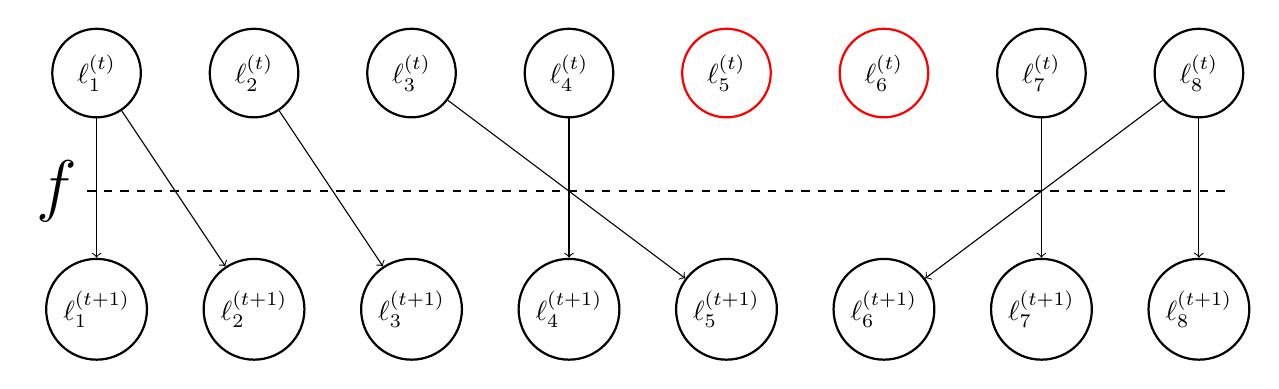
\begin{tikzpicture}
    \begin{scope}[auto, every node/.style={draw=black,circle,thick,minimum size=3.2em}]
        \node (A_1) at (0, 0) {$\ell^{(t + 1)}_1$};
        \node (A_2) at (2, 0) {$\ell^{(t + 1)}_2$};
        \node (A_3) at (4, 0) {$\ell^{(t + 1)}_3$};
        \node (A_4) at (6, 0) {$\ell^{(t + 1)}_4$};
        \node (A_5) at (8, 0) {$\ell^{(t + 1)}_5$};
        \node (A_6) at (10, 0) {$\ell^{(t + 1)}_6$};
        \node (A_7) at (12, 0) {$\ell^{(t + 1)}_7$};
        \node (A_8) at (14, 0) {$\ell^{(t + 1)}_8$};

        \node (B_1) at (0, 3) {$\ell^{(t)}_1$};
        \node (B_2) at (2, 3) {$\ell^{(t)}_2$};
        \node (B_3) at (4, 3) {$\ell^{(t)}_3$};
        \node (B_4) at (6, 3) {$\ell^{(t)}_4$};
        \node (B_7) at (12, 3) {$\ell^{(t)}_7$};
        \node (B_8) at (14, 3) {$\ell^{(t)}_8$};

        \node[draw=red] (B_5) at (8, 3) {$\ell^{(t)}_5$};
        \node[draw=red] (B_6) at (10, 3) {$\ell^{(t)}_6$};
    \end{scope}

    \begin{scope}
        \node (C_1) at (-0.5, 1.5) {\Huge$f$};
        \node (C_2) at (14.5, 1.5) {};
        \draw[thick, dashed] (C_1) -- (C_2);
    \end{scope}

    \begin{scope}[every edge/.style={draw=black}]
        \path[->] (B_1) edge (A_2);
        \path[->] (B_1) edge (A_1);
        \path[->] (B_2) edge (A_3);
        \path[->] (B_3) edge (A_5);
        \path[->] (B_4) edge (A_4);
        \path[->] (B_8) edge (A_6);
        \path[->] (B_8) edge (A_8);
        \path[->] (B_7) edge (A_7);
    \end{scope}
\end{tikzpicture}}
    \caption{An example of population $\pi^{(t)}$ evolving to $\pi^{(t+1)}$ under the Wright-Fisher model.
    Each individual $\ell^{(t+1)}_i \in \pi^{(t+1)}$, represents the result of applying some mutation function $f$ to
    some individual in $\ell^{(t)}_i$.
    Note that there are two individuals that do not advance to $\pi^{(t+1)}$: $\ell^{(t)}_5$ and $\ell^{(t)}_6$.}
    \label{fig:wrightFisherEvolution}
\end{figure}

\subsection{Average Time Until $n$ Individuals Coalesce: $\overbar{t}$}
\label{subsec:averageTimeUntilNIndividualsCoalesce}
The next question that follows is, ``What is $\overbar{t}$?''.
The naive approach (but most correct) is to keep track of the evolutionary history for all populations.
This however requires (a) storage for the evolutionary tree formed and (b) an expensive search as we move forward for
each generation.
A compromise that avoids this search and storage increase is to fix $\overbar{t}$ to some value, a time where most
populations have a common ancestor shared across the entire population.

\begin{figure}[t]
    \centering
    \subfloat{{ \usetikzlibrary{decorations.pathreplacing}
\begin{tikzpicture}
    \begin{scope}[auto, every node/.style={draw=black,circle,thick,minimum size=1em}]
        \foreach \x in {1,...,5}
            \foreach \y in {0,...,8}{
                \node (\x\y) at (\x,\y) {};
            }
    \end{scope}

    \begin{scope}[auto, every node/.style={draw=black,circle,thick,minimum size=1em,fill=blue}]
        \node (A_1) at (3,0) {};
        \node (A_2) at (5,0) {};

        \node (B_1) at (1,1) {};
        \node (B_2) at (4, 1) {};

        \node (C_1) at (2, 2) {};
        \node (C_2) at (5, 2) {};

        \node (D_1) at (2, 3) {};
        \node (D_2) at (3, 3) {};

        \node (E_1) at (3, 4) {};
        \node (F_1) at (1, 5) {};
        \node (G_1) at (4, 6) {};
        \node (H_1) at (2, 7) {};
        \node (I_1) at (3, 8) {};
    \end{scope}

    \begin{scope}[every edge/.style={draw=black,thick}]
        \path (A_1) edge (B_1);
        \path (A_2) edge (B_2);
        \path (B_1) edge (C_1);
        \path (B_2) edge (C_2);
        \path (C_1) edge (D_1);
        \path (C_2) edge (D_2);
        \path (D_1) edge (E_1);
        \path (D_2) edge (E_1);

        \path (E_1) edge (F_1);
        \path (F_1) edge (G_1);
        \path (G_1) edge (H_1);
        \path (H_1) edge (I_1);
    \end{scope}

    \node (T_A) at (0.5, -0.25) {};
    \node (T_B) at (0.5, 4.25) {};
    \draw[decoration={calligraphic brace,amplitude=10pt},decorate,line width=1.2pt]
    (T_A) -- node[anchor=east, xshift=-8pt] {$\bar{t} = N$} (T_B);
\end{tikzpicture} }}
    \qquad \qquad \qquad
    \subfloat{{ \usetikzlibrary{decorations.pathreplacing}
\begin{tikzpicture}
    \begin{scope}[auto, every node/.style={draw=black,circle,thick,minimum size=1em,fill=blue}]
        \node (A_1) at (1,0) {};
        \node (A_2) at (5, 0) {};
        \node (A_3) at (3, 4) {};
    \end{scope}

    \begin{scope}[every edge/.style={draw=black,thick}]
        \path (A_1) edge (A_3);
        \path (A_2) edge (A_3);
        \node (A_4) at (3, 8.5) {};
        \path (A_3) edge (A_4);
    \end{scope}

    \node (T_A) at (0.5, -0.25) {};
    \node (T_B) at (0.5, 4.25) {};
    \draw[decoration={calligraphic brace,amplitude=10pt},decorate,line width=1.2pt]
    (T_A) -- node[anchor=east, xshift=-8pt] {$\bar{t} = N$} (T_B);
\end{tikzpicture} }}
    \caption{A coalescent buried in some forward simulation.}
    \label{fig:coalescentBuried}
\end{figure}

Let us start with $n=2$ individuals and two generations: $t, t-1$.
In a Wright-Fisher population, the probability $p(2, t-1)$ that any two individuals in $\pi^{(t)}$ share the same
parent from $\pi^{(t-1)}$ is:
\begin{equation}
    p(2, t-1) = \frac{1}{N}
\end{equation}
Consequently, the probability $q(2, t-1)$ that two individuals do not share a parent from $\pi^{(t-1)}$ is:
\begin{equation}
    q(2, t-1) = 1 - \frac{1}{N}
\end{equation}
The probability that two individuals do not share a parent in $\pi^{(t-1)}$, but do have a common ancestor
in $\pi^{(t-2)}$ is:
\begin{equation}
    p(2, t-2) = q(2, t-1) \cdot \frac{1}{N} = \frac{1}{N} \cdot \left(1 - \frac{1}{N}\right)
\end{equation}
If we ask the same question but for $\pi^{(t-3)}$, we get
$p(2, t-3) = \frac{1}{N} \cdot  \left(1 - \frac{1}{N}\right)^2$.
Noting that this probability $p$ is geometrically distributed, we can generalize $p$ for having two individual share a
common ancestor $y$ generations ago:
\begin{equation}
    p(2, t-y) = \frac{1}{N} \cdot \left(1 - \frac{1}{N}\right)^{y-1}
\end{equation}
with $p(2, t-y)$ having mean $E_2 = N$.
The mean $E_2$ is interpreted as the expected number of generations until $n=2$ individual \emph{coalesce}.

Now we look at the probability that $n=3$ individuals in $\pi^{(t)}$ share a parent from $\pi^{(t-1)}$.
Here, we asking how many pairs can be formed with $n=3$ out of the entire population:
\begin{equation}
    p(3, t-1) = \frac{3}{N}
\end{equation}
Given $n=4$ individuals, the probability that any of the four share a parent in $\pi^{(t-1)}$ is
$p(4, t-1) = \frac{6}{N}$.
We generalize $p$ for a coalescent event occurring with $n$ individuals in the previous generation as such:
\begin{equation}
    p(n, t-1) = \frac{\binom{n}{2}}{N}
\end{equation}
For $y$ generations, the general form of $p$ is given~\cite{hudsonGeneGenealogiesCoalescent1990}:
\begin{equation}
    p(n, t-y) = \frac{\binom{n}{2}}{N} \cdot \left(1 - \frac{\binom{n}{2}}{N}\right)^{y-1}
\end{equation}
with $p(n, t-y)$ having mean:
\begin{equation}\label{eq:expectedMeanCoa}
    E_n = \frac{N}{\binom{n}{2}}
\end{equation}
The mean $E_n$ is interpreted as the expected number of generations until two out of $n$ individuals coalesce.

Going back to our original question, what is the \emph{average} time until $n$ individuals share a common ancestor?
Let us start with the average time until two individuals coalesce: $E_2 = N$ generations.
The average time until three individuals coalesce is the average time until any two individuals coalesce \emph{plus} the
average time until coalescence occurs in any three individuals.
For all $n$ individuals, this average time must be greater than:
\begin{equation}
    \begin{aligned}
        \overbar{t} >& \sum_{i=2}^{n} E_i \\
        \overbar{t} \gtrapprox& \ 2N
    \end{aligned}
\end{equation}

\subsection{Effective Population $\hat{\pi}$ Sampling}\label{subsec:effectivePopulationPiSampling}
To circumvent the inefficient space strategy of tracking all lineages formed, we instead chose to simulate to a fixed
number of generations $\overbar{t} = 2N$.
Let $\hat{\pi}$ represent a population of individuals who coalesce.
We have to choose a select few individuals, or \emph{sample} from $\hat{\pi}$ to obtain $\tilde{\pi}$.
The data that we are comparing to our generated repeat units has been collected in samples, not entire populations.
The problem here, is that our sample of $n$ individuals may not share a common ancestor.

The simplest approach to mitigate the impact of this problem is to run our simulation process longer than the expected
time to coalescence.
This allows us to strengthen our belief that more individuals in $\pi^{(2N)}$ have coalesced.
We denote this additional running time as $t_\epsilon$, a tunable parameter of our procedure.
This makes our minimum running time:
\begin{equation}
    \overbar{t} = 2N + t_\epsilon
\end{equation}
Once we have run the evolution process for $\overbar{t}$ generations, we sample randomly $n$ individuals.

\subsection{Forward Evolution Algorithm}\label{subsec:forwardEvolutionAlgorithm}
\begin{algorithm}[t]
    \SetAlgoLined
    \DontPrintSemicolon
    \Fn{ForwardSimulator \ {$(\ell^{(1)}, N, n, t_{\epsilon}, f(\ell))$}} {
        \KwIn{a common ancestor $\ell^{(1)}$, population size $N$, sample size $n$, extra running time $t_\epsilon$,
        a single-generation mutation function $f$}
        \KwOut{a sample from the resultant population $\tilde{\pi}$}
        $\pi^{(t-1)} \gets \{ \ell_1 \}$  \
        $\pi^{(t)} \gets \emptyset$ \;
        \For{$t \gets 2$ \KwTo $t_\epsilon + 2N - 1$} {
            \For{$j \gets 1$ \KwTo $N$} {
                $\pi^{(t)} \gets \pi^{(t)} \cup \{f$(a randomly selected $\ell$ from $\pi^{(t-1)} )\}$ \;
            }
            $\pi^{(t-1)} \gets \pi^{(t)}$ \;
            $\pi^{(t)} \gets \emptyset$ \;
        }
        $\tilde{\pi} \gets n$ random $\ell$ from $\pi^{(t-1)}$ \;
        \Return $\tilde{\pi}$ \;
    }
%    \textbf{end} \;
    \caption{Generate a sample of individuals who \emph{likely} share some common ancestors.}
    \label{alg:forwardEvolution}
\end{algorithm}

The function for forward evolution is presented in~\autoref{alg:forwardEvolution}, and described below.
\begin{enumerate}
    \item For simplicity, we treat our starting population $\pi^{(1)}$ as $N$ instances of some common ancestor
        $\ell^{(1)}$.
        All individuals in the output $\pi$ are expected to share one member from $\pi^{(1)}$, meaning that all other
        individuals in $\pi^{(1)}$ get thrown away.
        With this approach, we only need to worry about one parameter.
    \item Mutation is discussed in detail in~\autoref{ch:modelingMutation}.
        For now, we define $f(\ell)$ to be some function $f : \mathbb{M} \rightarrow \mathbb{M}$ which
        takes some repeat unit and returns another repeat unit.
    \item We start by defining our storage vectors, $\pi^{(t-1)}$ and $\pi^{(t)}$.
        These hold the ancestor and descendant generations respectively.
        Both are of size $N$, the effective population size.
    \item The simulation is run for $t_\epsilon + 2N$ generations.
        At each generation $t - 1$ we randomly sample $N$ individuals, apply our mutation function $f$, and store the
        resultant in descendant generation $\pi^{(t)}$.
        After this process, the current descendant generation $\pi^{(t)}$ becomes the next ancestor generation
        $\pi^{(t+1)}$ as we increment $t$.
    \item Once we have reached the end generation, we return $n$ randomly sampled individuals from the last generation.
\end{enumerate}

%The time complexity $T_\text{forward}$ of this algorithm is strictly bounded by $N$.
%The space complexity $S_\text{forward}$ is also strictly bounded by $N$:
%\begin{align}
%    T_\text{forward}(N) &\in \Theta(N^2) \\
%    S_\text{forward}(N) &\in \Theta(N)
%\end{align}

\section{Backward Simulation}\label{sec:backwardSimulation}
Forward simulation has the advantage of being incredibly straightforward to implement and apply complex generation to
generation models to.
The biggest disadvantages with this type of simulation though, are that (a) $2N^2$ individuals must
be generated per simulation and (b) several returned populations from the forward simulator will not coalesce.
In this section, we will go over backward simulation -- an approach that addresses both of these problems.

\subsection{Kingman's Coalescent Construction}\label{subsec:kingmanCoalescentConstruction}
As previously mentioned, the first drawback to forward simulation is the retention of individuals that do not exist in
the evolutionary tree of the latest generation.
Let $\mathcal{N}$ represent the total number of individuals we must simulate in order to produce a population sample of
size $n$.
For a population $\pi$ of size $|\pi| = N$, we can compute the minimum number of total individuals that we simulate
$\mathcal{N}^\star$:
\begin{equation}
    \mathcal{N}^\star = \sum_{i=1}^n i = \binom{n + 1}{2}
\end{equation}
When using forward simulation with $\mathcal{N}_{F} = 2N^2$, there exists a waste of
$\mathcal{N}_{waste}$ individuals created:
\begin{equation}
    \begin{aligned}
        \mathcal{N}_{{waste}} &= \mathcal{N}_{F} - \mathcal{N}^\star \\
        &= 2N^2 - \binom{n + 1}{2}
    \end{aligned}
\end{equation}
Given $N = 1,000, n = 100$, there exists $\mathcal{N}_{waste} = 1,994,950$.
Nearly two-million individuals are needlessly generated to produce only 100 end individuals.

\begin{figure}[t]
    \centering
    \subfloat{\usetikzlibrary{decorations.pathreplacing}
\begin{tikzpicture}
    \begin{scope}[auto, every node/.style={draw=black,circle,thick,minimum size=1em,fill=blue}]
        \node (A_1) at (1, 0) {};
        \node (A_2) at (2, 0) {};
        \node (A_3) at (3, 0) {};
        \node (A_4) at (4, 0) {};
        \node (A_5) at (5, 0) {};

        \node (B_1) at (1.5, 0.5*1.2) {};  % N = 5, 5 choose 2 = 10, 5 / 10 = 0.5
        \node (B_2) at (2.5, 0.5*1.2) {};
        \node (B_3) at (3.5, 0.5*1.2) {};
        \node (B_4) at (4.5, 0.5*1.2) {};

        \node (C_1) at (2, 1.33*1.2) {};  % N = 5, 4 choose 2 = 6, 5 / 6 = 0.83
        \node (C_2) at (3, 1.33*1.2) {};
        \node (C_3) at (4, 1.33*1.2) {};

        \node (D_1) at (2.5, 3*1.2) {};  % N = 5, 3 choose 2 = 3, 5 / 3 = 1.66
        \node (D_2) at (3.5, 3*1.2) {};

        \node (E_1) at (3, 8*1.2) {};  % N = 5, 2 choose 2 = 1, 5 = 5
    \end{scope}

    \begin{scope}[every edge/.style={draw=black,thick}]
        \path (A_1) edge (B_1);
        \path (A_2) edge (B_1);
        \path (A_3) edge (B_2);
        \path (A_4) edge (B_3);
        \path (A_5) edge (B_4);

        \path (B_1) edge (C_1);
        \path (B_2) edge (C_1);
        \path (B_3) edge (C_2);
        \path (B_4) edge (C_3);

        \path (C_1) edge (D_1);
        \path (C_2) edge (D_1);
        \path (C_3) edge (D_2);

        \path (D_1) edge (E_1);
        \path (D_2) edge (E_1);
    \end{scope}

    \node (T_A) at (0.5, -0.25) {};
    \node (T_B) at (0.5, 0.6+0.25) {};
    \draw[decoration={calligraphic brace,amplitude=5pt},decorate,line width=1.2pt]
    (T_A) -- node[anchor=east, xshift=-8pt] {$t_4 = N \cdot \binom{5}{2}^{-1}$} (T_B);

    \node (T_B2) at (0.5, 0.6) {};
    \node (T_C) at (0.5, 1.6+0.25) {};
    \draw[decoration={calligraphic brace,amplitude=5pt},decorate,line width=1.2pt]
    (T_B2) -- node[anchor=east, xshift=-8pt] {$t_3 = N \cdot \binom{4}{2}^{-1}$} (T_C);

    \node (T_C2) at (0.5, 1.6) {};
    \node (T_D) at (0.5, 3.6+0.25) {};
    \draw[decoration={calligraphic brace,amplitude=5pt},decorate,line width=1.2pt]
    (T_C2) -- node[anchor=east, xshift=-8pt] {$t_2 = N \cdot \binom{3}{2}^{-1}$} (T_D);

    \node (T_D2) at (0.5, 3.6) {};
    \node (T_E) at (0.5, 9.6+0.25) {};
    \draw[decoration={calligraphic brace,amplitude=5pt},decorate,line width=1.2pt]
    (T_D2) -- node[anchor=east, xshift=-8pt] {$t_1 = N \cdot \binom{2}{2}^{-1}$} (T_E);
\end{tikzpicture}}
    \qquad \qquad \qquad
    \subfloat{\usetikzlibrary{decorations.pathreplacing}
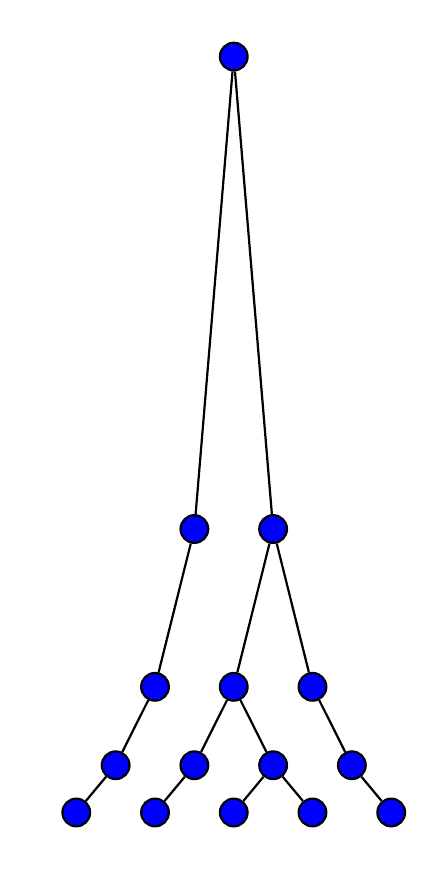
\begin{tikzpicture}
    \begin{scope}[auto, every node/.style={draw=black,circle,thick,minimum size=1em,fill=blue}]
        \node (A_1) at (1, 0) {};
        \node (A_2) at (2, 0) {};
        \node (A_3) at (3, 0) {};
        \node (A_4) at (4, 0) {};
        \node (A_5) at (5, 0) {};

        \node (B_1) at (1.5, 0.5*1.2) {};  % N = 5, 5 choose 2 = 10, 5 / 10 = 0.5
        \node (B_2) at (2.5, 0.5*1.2) {};
        \node (B_3) at (3.5, 0.5*1.2) {};
        \node (B_4) at (4.5, 0.5*1.2) {};

        \node (C_1) at (2, 1.33*1.2) {};  % N = 5, 4 choose 2 = 6, 5 / 6 = 0.83
        \node (C_2) at (3, 1.33*1.2) {};
        \node (C_3) at (4, 1.33*1.2) {};

        \node (D_1) at (2.5, 3*1.2) {};  % N = 5, 3 choose 2 = 3, 5 / 3 = 1.66
        \node (D_2) at (3.5, 3*1.2) {};

        \node (E_1) at (3, 8*1.2) {};  % N = 5, 2 choose 2 = 1, 5 = 5
    \end{scope}

    \begin{scope}[every edge/.style={draw=black,thick}]
        \path (A_1) edge (B_1);
        \path (A_2) edge (B_2);
        \path (A_3) edge (B_3);
        \path (A_4) edge (B_3);
        \path (A_5) edge (B_4);

        \path (B_1) edge (C_1);
        \path (B_2) edge (C_2);
        \path (B_3) edge (C_2);
        \path (B_4) edge (C_3);

        \path (C_1) edge (D_1);
        \path (C_2) edge (D_2);
        \path (C_3) edge (D_2);

        \path (D_1) edge (E_1);
        \path (D_2) edge (E_1);
    \end{scope}

    \node (T_A) at (0.5, -0.25) {};
    \node (T_B) at (0.5, 0.6+0.25) {};

    \node (T_B2) at (0.5, 0.6) {};
    \node (T_C) at (0.5, 1.6+0.25) {};

    \node (T_C2) at (0.5, 1.6) {};
    \node (T_D) at (0.5, 3.6+0.25) {};

    \node (T_D2) at (0.5, 3.6) {};
    \node (T_E) at (0.5, 9.6+0.25) {};
\end{tikzpicture}}
    \caption{Two variations of a Kingman's coalescent tree with $n = 5$.
    Note the decrease in edge length (i.e.\ time) as the depth of nodes increases.}
    \label{fig:coalescentTree}
\end{figure}

A backwards simulation reduces $\mathcal{N}_{waste}$ to 0 for all values of $n$ by only working with individuals
involved in a coalescent event.
Instead of working from generation to generation, this type of simulation works from one \emph{coalescent event} to
another.
This allows us to abstract away from generational time steps for now, and build a \emph{coalescent tree}.
More precisely, we are going to work with Kingman's coalescent trees.
These follow a structure similar to~\autoref{fig:coalescentTree}, varying only in which parent node connects two child
nodes.

To start, we define $\pi^{(t)}_i$ as the repeat unit associated with some individual $\ell$ in population $\pi$ at
generation $t$, and $v_j$ a node associated with this repeat unit, enumerated by $j$ for a set of
populations.
Let $V$ represent the set that holds all nodes used in an instance of a Kingman's coalescent.
$V$ can be thought of as all the nodes associated with the evolutionary tree, or graph, that we are building.

To state that some node $v_a$ is the direct descendant of $v_b$ is to use the following \emph{directed} edge:
\begin{equation}
    (v_a, v_b) \Leftrightarrow v_a \text{ directly descends from } v_b
\end{equation}
Building the set of directed weighted edges $E$ that connect our graph requires the conditions given below.
\begin{enumerate}
    \item For some edge $(v_a, v_b)$, $v_a$ must exist in a generation after $v_b$.
        This implies that $v_1$ is the sink of our graph and all nodes in the generation-to-be-sampled $\hat{\pi}$ are
        sources.
    \item For some edge $(v_a, v_b)$, both $v_a$ and $v_b$ must exist in the set of nodes associated with some instance
        of a Kingman's coalescent $V$.
    \item Recall that all individuals of a Kingman's coalescent at generation $t$ are copied into the following
        generation, with only one individual being copied twice.
        Let $V^{(t)}$ represent all nodes used in the Kingman's coalescent that exist in population $\pi^{(t)}$ at
        generation $t$.
        For all edges formed using $V^{(t+1)}$ and $V^{(t)}$, there exists only two edges $(v_a, v_b), (v_c, v_b)$ where
        the ancestor node $v_b$ is seen twice.
        For all other edges the descendant node must be unique \& from $V^{(t)}$, and the ancestor node must also be
        unique \& from the set $V^{(t+1)}$.
        This constraint is illustrated with the coalescent tree examples in~\autoref{fig:coalescentTree}.
    \item Each edge $(v_a, v_b)$ has an associated weight, representing the difference in generations between nodes
        $v_a$ and $v_b$.
        For an edge $e \in E$, this weight is found using the function $\tau : E \rightarrow \mathbb{Z}^+$.

\end{enumerate}

\subsection{Coalescent Repeat Unit Resolution}\label{subsec:coalescentRepeatLengthResolution}
Constructing the tree is the first step associated with obtaining a sample of $n$ individuals.
The next step is to determine the repeat units associated with some node $v_i \in V$.
We define the function $\lambda : E \rightarrow \mathbb{M}$ which resolves the repeat unit of some
individual of our coalescent tree given some edge $e \in E$, and our mutation function $f$.
For all edges $(v_i, v_j) \in E$, the repeat unit $\ell_i$ associated with node $v_i$ is given by running
$\ell_i$ through $f$ for a set number of generations to $v_j$.
The next question of interest is, ``How many generations do we apply $f$ for?''.

In~\autoref{sec:forwardSimulation}, we determined that the expected time between coalescent events for $n$ individuals
in a population of size $N$ (\autoref{eq:expectedMeanCoa}).
This number naturally emerged as a result of the Wright-Fisher evolution process, but we must manually define this time
with the coalescent abstraction.
Let $\tau_N(e)$ represent a function $\tau_N : E \rightarrow \mathbb{Z}^+$ that takes some edge $e$ as input and returns
the number of generations between the associated nodes.
The most common approach is to draw these generations from an exponential distribution with mean
$\frac{N}{\binom{\rho(e)}{2}}$~\cite{hudsonGeneGenealogiesCoalescent1990}:
\begin{align}
    e &= \text{ an edge } (v_i, v_j) \text{ connecting nodes } v_i \text{ and } v_j \\
    \tau_N(e) &\sim \exp\left(\frac{N}{\binom{\rho(e)}{2}}\right)
\end{align}
where $\rho(e)$ represents an additional function $\rho : E \rightarrow \mathbb{Z}^+$ that determines the working coalescent
event attached to some edge $e$.
$\rho(e)$ can also be thought of as a depth determination function for the incoming edge attached to $e$.

Starting from the ancestor node $v_1$, we perform a breadth-first search (BFS) to visit nodes of the same depth first
before moving to the next node.
Upon arrival, we apply the mutation process to each visited node and descend further down our tree.
This means that we perform our simulation in order of coalescent event, rather than lineage (which would require a
depth first search, or DFS).
Once we have visited each node, we return the repeat units associated with our leaves: $\{ \lambda (v) \mid v
\text{ is a leaf }\}$.

\subsection{Backward Evolution Algorithm}\label{subsec:backwardEvolutionAlgorithm}
\begin{algorithm}[t]
    \SetAlgoLined
    \DontPrintSemicolon
    \Fn{TwoStageBackwardSimulator \ {$(\ell^{(1)}, n, f, \tau_N)$}} {
        \KwIn{a common ancestor $\ell^{(1)}$, sample size $n$, a single-generation mutation function $f$, a generation
        determination function $\tau_N$}
        \KwOut{a sample from the resultant population $\tilde{\pi}$}
        $V \gets $ an empty $\binom{2N}{2}$ sized vector,
        $E \gets $ an empty $(\binom{2N}{2} - 1)$ sized vector \;

%        \;
        \For(\tcc*[f]{Stage 1: Construct the tree.}){$i \gets 2$ \KwTo $2n$} {
            $E' \gets $ an empty $i$ sized vector,
            $A \gets \{ a \mid a \in [\binom{i - 1}{2} + 1, \binom{i}{2}] \land i \in \mathbb{Z} \}$ \;
            \For{$j \gets \binom{i - 1}{2} + 1$ \KwTo $\binom{i}{2}$} {
                $E'[j] \gets (V[a'], V[i]),$ where $a'$ is randomly selected from $A$ \;
                $A \gets A - \{ a' \}$ \;
            }
            $E'[i + 1] \gets (V[a'], V[i + 1])$, where $ a' \text{ is randomly selected from } \{ a \mid a \in
            [1, \binom{i}{2}] \land i \in \mathbb{Z} \}$ \; \label{algline:coalescentEvent}
            $E[\binom{i}{2}:\binom{i + 1}{2}] \gets \hat{E}$ \;
        }

%        \;
        $V[1] \gets \ell_1$ \;
        \For(\tcc*[f]{Stage 2: Determine the repeat units.}){$i \gets 2$ \KwTo $| V |$} {
            $v' \gets $ the incoming node attached to $E[i]$ \;
            \For{$j \gets 1$ \KwTo $\tau_N(e)$} {
                $v' \gets f(v')$ \;
            }
            $V[i + 1] \gets v'$ \;
        }

        \Return $V[\binom{n - 1}{2} + 1:\binom{n}{2}]$ \;
    }
%    \textbf{end} \;
    \caption{Generate a sample of individuals who share a common ancestor from some effective population.}
    \label{alg:twoStageBackwardEvolution}
\end{algorithm}

The function for backward evolution is presented in~\autoref{alg:twoStageBackwardEvolution}, and described below:
\begin{enumerate}
    \item There exist two stages here: the tree construction phase and the repeat unit determination phase.
        For the scope of this project it makes more sense to combine these phases and reduce our running time, however
        separating the two allows us to build more complex demographic models in the future
        (see~\autoref{ch:conclusion}).
    \item We use vector and index notation to represent our node and edge sets $V, E$.
        This is a more natural notation, and avoids having to explicitly specify $\lambda$.
        To specify consecutive vector elements (or \emph{slices}), the $[a:b]$ notation is used.
        Here, $a$ specifies the starting index of our vector (inclusive) and $b$ specifies the end index of our
        vector (inclusive).
    \item Contrary to the name ``backward simulation'', we build our tree top-down, or from ancestor to descendant.
        The working section of vectors $V, E$ for a given iteration $i$ is specified by the $i - 1$'th and $i$'th
        triangle number.
        To build the edge vector, we randomly from $\left[\binom{i}{2} + 1, \binom{i}{2} + 2, \ldots,
        \binom{i + 1}{2}\right]$
        \emph{without} replacement.
        This ensures that all ancestors advance to the next coalescent event.
        To replicate the coalescent event itself, we randomly select one ancestor to yield two descendants by generating
        an additional edge (see~\autoref{algline:coalescentEvent}).
    \item To determine the repeat unit (i.e.\ populate $V$), we move back to top and evolve down.
        Starting from the given common ancestor, we perform BFS by visiting the incoming nodes attached to edges in
        the order they were created in.
        Maintaining this order allows us to avoid having to specify the depth determination function $\rho(e)$.
        For each incoming node $v'$ attached to edge $e$, we applying our mutation process $\tau_N(e)$ times.
        The result is saved the the outgoing node attached to $e$.
        This is repeated for all edges.
    \item We return the leaves associated with our tree: the last $n$ elements of the $V$ vector.
\end{enumerate}

%The longest operation of this algorithm is the
%The time complexity $T_\text{backward}$ of this algorithm
%The time complexity $T_\text{forward}$ of this algorithm is strictly bounded by $N$.
%The space complexity $S_\text{forward}$ is also strictly bounded by $N$:
%\begin{align}
%    T_\text{forward}(N) &\in \Theta(N^2) \\
%    S_\text{forward}(N) &\in \Theta(N)
%\end{align}